\section{Scope, Genealogy, and Review Landscape}
\label{sec:background}

Medical world modeling did not emerge from a single technical lineage. The term now sits at the intersection of general world models, longitudinal clinical prediction, digital twins, causal treatment modeling, model-based decision making, and embodied medical systems. These traditions share an interest in change over time, but they disagree about what must be represented, whether actions need to be executable, and what evidence turns a plausible simulation into a clinically meaningful one. This section locates those traditions before the capability analysis. Its purpose is not to award a capability level to review or position papers, but to make clear which conceptual commitments the implemented literature inherits.

\subsection{General World Models and Model-Based Decision Making}

General world-model surveys describe a broad family rather than a single architecture. Some emphasize predictive state representations, others generative environments, and others the operational use of learned dynamics for planning or control. Surveys spanning foundation models, video generation, and autonomous driving show how easily the term expands from ``a model that predicts the world'' to ``a system that supports interaction'' \citep{Zhu2024IsSoraWorld,Ding2025UnderstandingWorldPredicting,Feng2025SurveyWorldModels}. That breadth is productive, but it also explains why terminology alone cannot organize the medical literature. A representation learner, a video generator, and a planner may all be called world models while answering different scientific questions.

Medicine makes the distinction consequential. In games or engineered simulators, the action set and transition rules are usually defined by the environment. Clinical records instead mix patient evolution with measurement, documentation, clinician behavior, access, and local practice. An accurate next-event model can therefore reproduce the care process without identifying how the patient would respond to a different intervention. The useful inheritance from general world models is not a particular backbone. It is the decomposition into state, transition, action, outcome, and model use, together with the recognition that rollout error can alter downstream decisions.

\subsection{Medical World-Model Surveys, Positions, and Definitions}

The medical-world-model literature increasingly frames the field as a progression from passive representation and forecasting toward intervention-conditioned simulation and planning. Recent reviews and perspectives describe combinations of patient state, temporal dynamics, intervention interfaces, multimodal observations, and decision support \citep{Saeed2026MedicalWorldModel,Liu2026MedicalWorldModelsReview,Feng2026StaticRiskDynamic,Wang2026TowardsBiomedicalWorldModels}. Their common contribution is to reject a purely static account of medical AI. Their definitions are not identical, however. Some include predictive state encoders within the world-model family, whereas others reserve the term for explicit dynamics or action-responsive rollout. Some treat planning as the culmination of the same ladder, whereas others distinguish simulation from policy optimization.

Adjacent clinical surveys broaden this genealogy. Computational modeling and simulation have long been evaluated as clinical tools, while clinical pharmacology and diagnostic specialties have developed their own accounts of how AI can support or distort decisions \citep{Johnson2023potentialpitfallsartificial,Walter2021Howartificialintelligence,Lesage2023Mappingusecomputational}. Virtual-brain work shows how a patient-specific computational model can connect neuroscience and clinical use without relying on contemporary world-model branding \citep{Wang2024VirtualBrainTwins}. Medical robotics and embodied-AI perspectives place the emphasis elsewhere: autonomy depends on coupling perception, interaction, human oversight, and task execution, not merely producing a realistic future frame \citep{Navab2026DyadicPartnershipDp,Liu2025ScreensScenesSurvey}. Taken together, these sources support a broad scope but also motivate a stricter operational definition. The present survey treats them as intellectual and application lineages; capability is assigned only to implemented task contracts.

\subsection{General Medical Digital Twins and Virtual Patients}

Digital twins form the largest adjacent review literature. Consensus, scoping, and broad healthcare reviews commonly describe a virtual counterpart that is linked to a physical patient or system and updated with observations over time \citep{Sun2022DigitalTwinMedicine,Cellina2023DigitalTwinsNew,Wang2023Opportunitieschallengesdigital,Vall_e2023Digitaltwinhealthcare,Sun2023Digitaltwinhealthcare,Katsoulakis2024Digitaltwinshealth}. The update relation is important: it separates an enduring twin from a one-time patient model. Yet the literature varies in how strictly this requirement is applied. Some accounts use digital twin for a patient-specific simulator, others for a predictive dashboard, and others for a broader data and decision infrastructure.

The proposed information pathways are correspondingly diverse. Reviews discuss imaging-derived anatomy, multimodal clinical data, omics, connected devices, wearables, laboratory measurements, and synthetic data as possible sources for twin construction and updating \citep{ukaniszyn2024DigitalTwinsGenerated,Papachristou2024DigitalTwinsAdvancements,Padoan2024Dynamicmirroringunveiling,Vall_e2024EnvisioningFuturePersonalized,Johnson2024DigitalTwinsHealthcare,Niarakis2024ImmuneDigitalTwins}. These sources can improve state estimation, but their presence does not establish a dynamic model. A multimodal patient representation may initialize a twin while remaining unable to forecast, simulate an action, or compare decisions.

Recent consensus and review work increasingly recognizes this distinction. Imaging, monitoring, IoT, and AI can support personalization, but a credible twin also needs a specified transition, an update rule, uncertainty, and validation tied to its intended use \citep{Iqbal2025consensusstatementon,Zhao2025Currentprogressdigital,Rudsari2025Digitaltwinshealthcare,Ooka2025EraPreemptiveMedicine,Saratkar2025Digitaltwinpersonalized,Kabir2025Digitaltwinshealthcare}. A similar issue arises at the system boundary. A twin may represent a patient, an organ, a surgical environment, a laboratory process, or a healthcare operation. These are legitimate objects, but they imply different states, actions, horizons, and outcomes.

The newest literature also connects digital twins to large language models, world models, simulation-based monitoring, assisted surgery, and complex-systems medicine \citep{Nadeem2025comprehensivereviewdigital,Sad_e2025Medicaldigitaltwins,Asciak2025Digitaltwinassisted,Domenico2025ChallengesOpportunitiesDigital,Zhou2026DigitalTwinAi,Babu2026HumanDigitalTwins}. This convergence is conceptually useful because it highlights missing components in both directions. World-model systems often lack patient-specific calibration and repeated updating; digital-twin proposals often specify a system architecture without implementing an action-sensitive transition. We therefore treat digital twin as a system-form overlay that can occur at any capability level, not as a sixth level and not as evidence of capability by name.

\subsection{Disease- and Organ-Specific Digital-Twin Literatures}

Disease-specific reviews make the value and limits of digital-twin language more concrete. Oncology work emphasizes adaptive treatment, multiscale tumor physiology, radiopharmaceutical therapy, treatment toxicity, and patient-specific response \citep{Karaman2025Fromdatadriven,John2025systematicreviewAI,Shen2025Fromvirtualreality,Omolayo2022DigitalTwinFrameworks,Thiong_o2022DigitalTwinTechnology,Rahmim2022Theranosticdigitaltwins,Wang2024Fromvirtualpatients,Witt2026DigitalTwinsCatalysts,Elsayed2026DigitalTwinModels}. These applications have clinically meaningful actions and outcomes, but they also face long horizons, treatment switching, censoring, and incomplete observation of alternative outcomes. The central challenge is consequently not whether a tumor can be rendered or parameterized, but whether the twin's response to a changed regimen is supported.

Cardiovascular twin reviews are often closer to mechanistic modeling. They connect anatomy, electrophysiology, hemodynamics, imaging, and therapy planning across atrial fibrillation and broader cardiovascular care \citep{Coorey2022healthdigitaltwin,Trayanova2023Updigitalpersonal,Thangaraj2024Cardiovascularcaredigital,Sel2024BuildingDigitalTwins,Karakasis2025DigitalTwinModels}. This structure offers interpretable state variables and intervention pathways. It also exposes parameter-identification and uncertainty problems: a model can be physiologically plausible at the population level while remaining weakly individualized for a specific patient.

Neurological, immune, musculoskeletal, and dermatological reviews illustrate still other meanings of a twin. Multiple-sclerosis and migraine work focuses on disease state and progression; immune-twin roadmaps emphasize multiscale and adaptive systems; orthopedic and arthroscopic reviews foreground geometry, mechanics, and procedural interaction; dermatology highlights observation and longitudinal monitoring \citep{Voigt2021DigitalTwinsMultiple,Gazerani2023IntelligentDigitalTwins,Laubenbacher2022Buildingdigitaltwins,Diniz2025Digitaltwinsystems,Bjelland2022TowardDigitalTwin,Akbarialiabad2024Digitaltwinsdermatology}. These literatures should not be collapsed into one application category. They are better compared by what is twinned, how it is updated, which actions are exposed, and what evidence supports the resulting prediction or decision.

\subsection{In Silico Trials, Verification, and Translation of Digital Twins}

A second digital-twin lineage is organized around evidence rather than organ system. Mechanism-based oncology, in silico trials, and AI-enabled twins raise questions about model qualification, verification, uncertainty, ethics, regulation, and implementation \citep{Wu2022Integratingmechanismbased,Strigari2025ComputationalNuclearOncology,Alharthi2025AIpoweredsilico,Samei2025FutureSilicoTrials}. These questions become more stringent as the intended use moves from explanation or training toward patient-specific treatment selection. A model may be useful for hypothesis generation without being qualified to replace a comparator arm or recommend care.

Meta-review and verification literature further shows that ``validation'' is not one operation \citep{Ringeval2025AdvancingHealthCare,Sel2025SurveyVerificationValidation,Glinkowski2026DigitalTwinsOrthopedics}. Numerical verification, biological plausibility, agreement with retrospective observations, external transportability, workflow utility, and decision impact support different claims. This observation directly motivates SATO-V: validation must be attached to the state, transition, action response, outcome, and intended decision, rather than reported as a generic property of the entire system.

\subsection{Longitudinal, Causal, and Model-Based Clinical Traditions}

Other adjacent literatures contribute pieces that digital-twin and world-model papers often leave implicit. EHR foundation-model critiques emphasize that longitudinal scale does not by itself recover patient dynamics, because records reflect coding and care processes \citep{Wornow2023shakyfoundationslarge}. Treatment-effect reviews make the identification problem explicit: individualized predictions under alternative interventions require assumptions about confounding, overlap, censoring, and temporal treatment assignment \citep{Bica2020FromRealWorld,Li2024Largepretrained}. Medical-world-model reviews that explicitly connect prediction, counterfactual reasoning, and planning help bring these concerns into the same conversation \citep{Qazi2025BeyondGenerativeAI}.

These traditions are complementary but non-interchangeable. A trajectory model can forecast the observed record without supporting intervention; a causal estimator can compare treatments without learning a general simulator; a model-based policy can optimize against learned dynamics without identifying patient-specific counterfactual effects. The survey therefore does not force them onto a cumulative maturity ladder. It asks which contract each implemented system satisfies and then evaluates the evidence needed for that contract.

\subsection{Competitive Positioning of This Survey}

Existing surveys provide valuable architecture, application, digital-twin, or capability maps. Our organizing choice is narrower: capability is the sole primary taxonomy, while paper role, clinical application, architecture, modality, and validation remain separate descriptors. Review, perspective, and conceptual papers establish genealogy and definitions but do not enter capability prevalence. General world models supply comparators but do not count as medical implementations. Digital twins are analyzed by implemented function rather than branding.

The second distinction is evidential. Papers are assigned according to the strongest implemented task contract, not the highest-level phrase in a title or discussion. SATO-V identifies where interpretation becomes uncertain: state, action, transition, outcome, or validation. This permits a constructive reading of the literature. A treatment-conditioned generator can be recognized as an action-responsive simulator without being credited with an identified treatment effect; a planner can be recognized as model-based without being treated as clinically valid. Detailed retrieval, coding, adjudication, and denominator rules are reported in Appendices~\ref{app:protocol} and~\ref{app:coding}.

Figure~\ref{fig:temporal-roadmap} provides a selective temporal view of representative lineages. It is an orientation device rather than an exhaustive chronology or a ranking.

\begin{figure}[t]
\centering
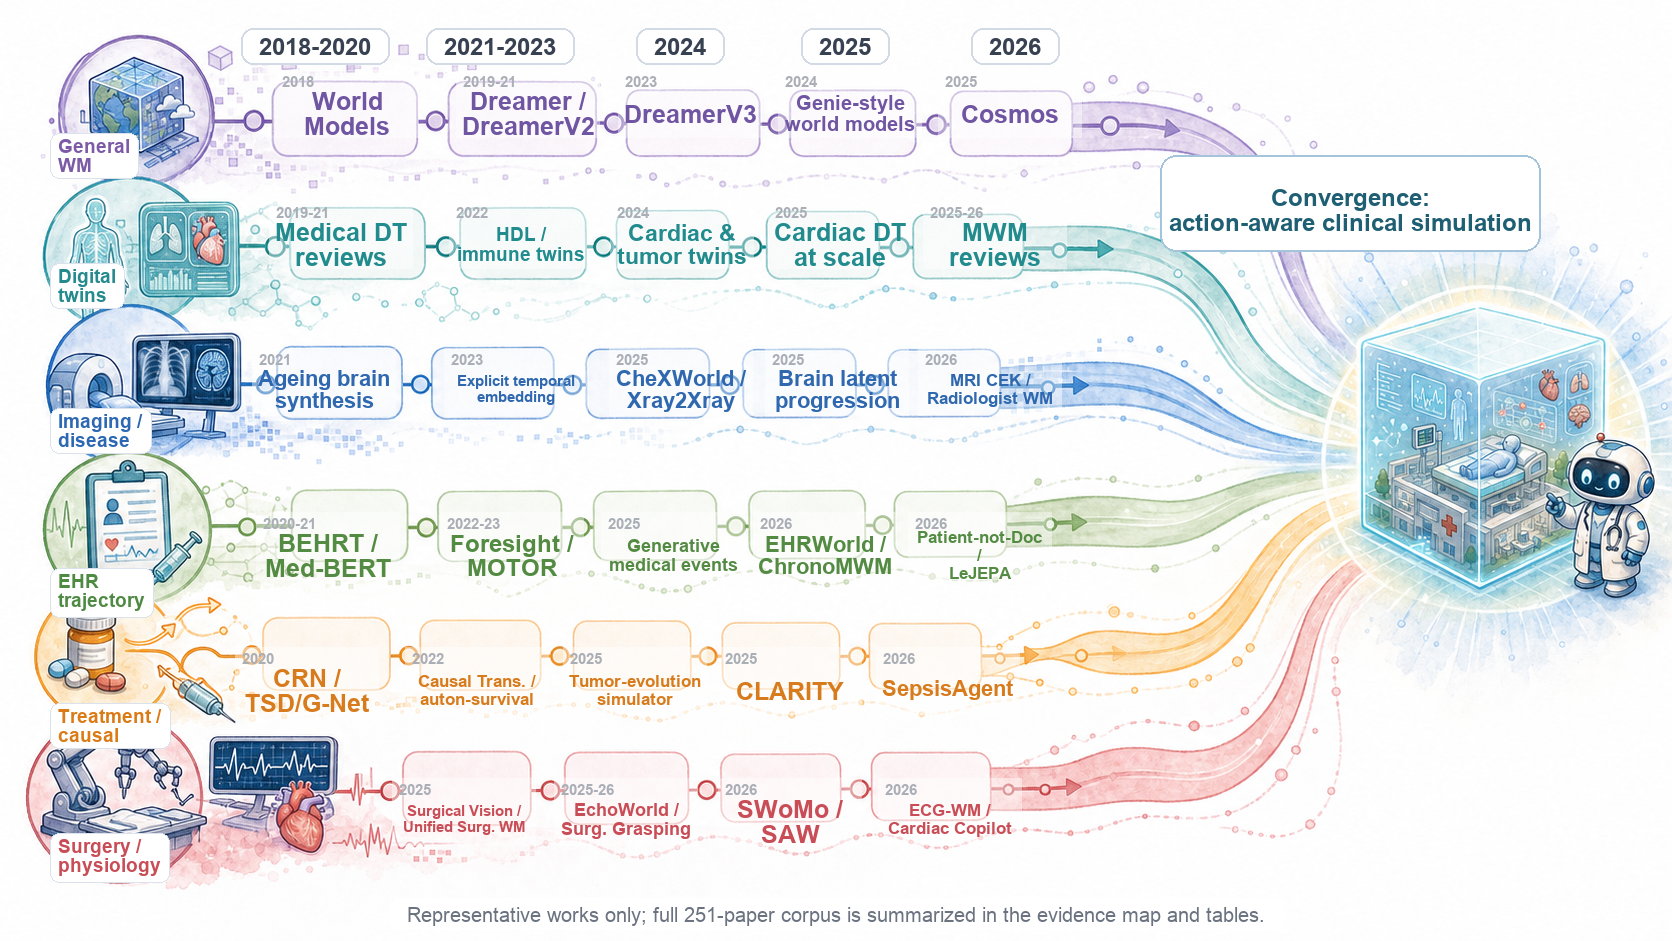
\includegraphics[width=\linewidth]{figures/fig_temporal_roadmap_imagegen_v1.png}
\caption{Temporal roadmap of representative works. Selected papers are arranged by approximate time and lineage: general world-model backbones, medical digital twins and reviews, imaging and disease-progression models, EHR trajectories, treatment and causal modeling, and surgical or physiological systems. The selection is illustrative rather than exhaustive.}
\label{fig:temporal-roadmap}
\end{figure}

